\documentclass[aspectratio=169]{beamer}
%\usetheme{Warsaw}
%AnnArbor, CambridgeUS, 
%\usecolortheme{beaver}
%\usetheme{seahorse}
\usetheme{Madrid}
\definecolor{pistachio}{rgb}{0.55, 0.77, 0.65}
\usecolortheme[named=pistachio]{structure} % Sample dvipsnames color


\usepackage[utf8]{inputenc}
\usepackage[portuguese]{babel}
\usepackage{graphicx}
%\usepackage{newtxtext,newtxmath}
\graphicspath{{imagens/}}
\usepackage{threeparttable}
\usepackage{tikz}
\geometry{}
\usepackage{multirow}
\usepackage{ragged2e}
\usepackage{subfig}
\setbeamercolor{block title}{bg=black!60,fg=white}
\usepackage{multicol}
\usepackage{tabularx}
\setbeamertemplate{itemize item}[square]
\setbeamertemplate{itemize subitem}[circle]
\setbeamertemplate{itemize subsubitem}[circle]
\setbeamercolor{itemize item}{fg=gray}
\setbeamercolor{itemize subitem}{fg=gray}
\setbeamercolor{itemize subsubitem}{fg=gray}
\setbeamertemplate{enumerate items}[square]
\setbeamercolor{item projected}{bg=gray!70!black,fg=white}
\usepackage[font=footnotesize,labelfont=bf]{caption}

\begin{document}
\title[Universidade Federal de Alfenas -- UNIFAL-MG]{Uma introdução à econometria espacial}

\author{Walef Machado de Mendonça}
\institute{PPGEAB}
\date{20 de Abril de 2021}

\begin{frame}{}
	\titlepage
\end{frame}

\begin{frame}{Introdução}
    
	\begin{itemize}
		\item A econometria espacial tem como objetivo \textbf{especificar}, \textbf{estimar}, \textbf{testar} e \textbf{prever} modelos teóricos influenciados pelos efeitos espaciais (ALMEIDA, 2012).
		\vspace{0.25cm}
		\item Na econometria espacial as observações representam regiões. Ex.: bairros, distritos, setores censitários, regiões urbanas etc
		\vspace{0.25cm}
		%\item 
	\end{itemize}

	\begin{figure}
		\small
		{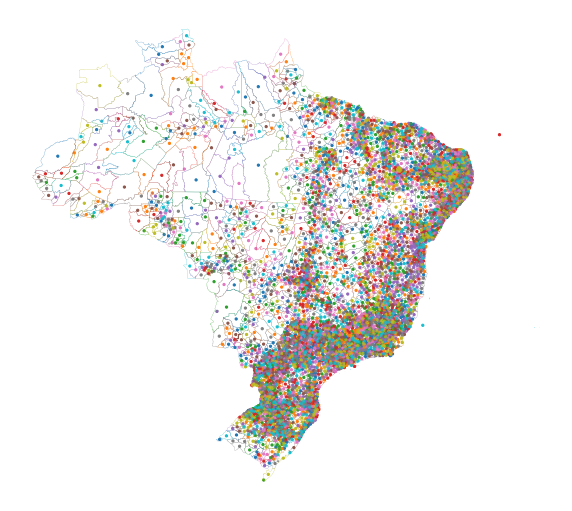
\includegraphics[width=0.25\textwidth]{img/inf_1.png}}\hspace{0.2cm}
		{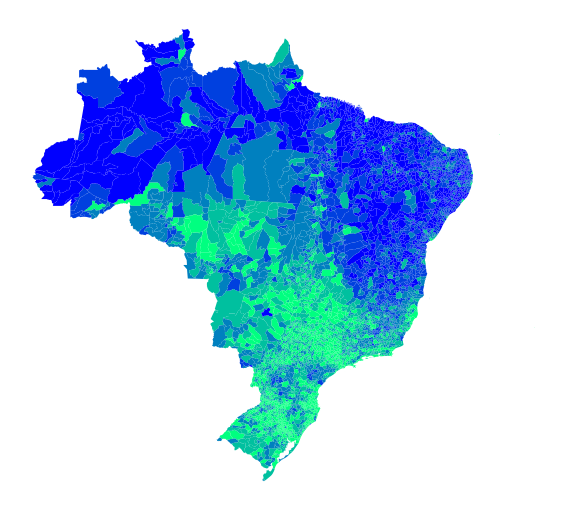
\includegraphics[width=0.25\textwidth]{img/inf_2.png}}\hspace{0.2cm}
	\end{figure}
\end{frame}

\begin{frame}{Introdução}
Geralmente a estrutura espacial contribui para a modelagem de duas formas:
\vspace{0.5cm}
		\begin{enumerate}
		    \item O processo gerador dos dados é explicitamente espacial. (ex.: preços de casas) $\rightarrow$ a geografia é uma variável e contribui \textbf{diretamente} para o modelo.
		    \item Uma alternativa é utilizar a localização espacial como uma variável \textbf{instrumental}. (ex.: o erro é maior em algumas áreas do que em outras)
		\end{enumerate}
\end{frame}

\begin{frame}{As hipóteses de Gauss-Markov}
	\begin{block}{}
	    \begin{equation}
        y = X\beta + \varepsilon
    \end{equation}
    \end{block}
    \begin{enumerate}
        \item \textbf{Lineariedade dos parâmetros}
        
        \item \textbf{Não colinearidade perfeita}
        
        \item \textbf{Média condicional zero}
        $$ \mathbb{E}(\varepsilon_i| X)=0$$
        
        \item \textbf{Homocedasticidade}
        $$Var(\varepsilon|X) = \sigma^2$$
        
        \item \textbf{Independência dos Erros}
        $$\mathbb{E}(\varepsilon_i \varepsilon_j | X) = 0  \text{ para } i \neq j$$
    \end{enumerate}
\end{frame}

\begin{frame}{Efeitos espaciais}
	\begin{itemize}
		\item \textbf{Dependência espacial}
		\vspace{0.5cm}
		\begin{itemize}
		    \item As unidades de corte transversal -- domicílios, municípios, regiões -- não são independentes entre si.
		    \item O valor de uma variável numa região $i$, $y_i$, depende do valor dessa mesma variável nas regiões vizinhas $j$, $y_j$. 
		\end{itemize}
		\vspace{0.5cm}
		\begin{block}{}
		    $$y_i = f(y_j,X), \quad i,j = 1,\dots, n \quad\text{e}\quad i\neq j$$
		\end{block}
		\vspace{0.25cm}
		$$ y_1 = \rho_2 y_2 + \beta X_1 +\varepsilon_1$$ 
	\end{itemize}
	\vspace{0.5cm}
\end{frame}

\begin{frame}{Efeitos espaciais}
	\begin{itemize}
		\item \textbf{Heterogeneidade espacial}
		\vspace{0.5cm}
		\begin{itemize}
			\item Ocorre quando há instabilidade estrutural através das regiões $\rightarrow$ diferentes respostas dependendo da localidade.
			\vspace{0.5cm}
			\begin{block}{}
			    $$y_i = f_i(X_i,\beta_i,\xi_i) \quad \xi_i \sim (0,\Omega)$$
			\end{block}
		\end{itemize}
	\end{itemize}
	\vspace{0.5cm}
\end{frame}

\begin{frame}{Os efeitos espaciais e as hipóteses de Gauss-Markov}
    \begin{enumerate}
        \item \textbf{Lineariedade dos parâmetros}
            \begin{itemize}
                \item Na presença de heterogeneidade espacial deve-se alterar a especificação do modelo para permitir que os coeficientes sejam variáveis de acordo com a localização do fenômeno.
            \end{itemize}
        \vspace{0.5cm}
        \item \textbf{Não colinearidade perfeita}
            \begin{itemize}
                \item Essa hipótese continua válida. Porém, ao se utilizar a defasagens espaciais a colnearidade pode aumentar. 
            \end{itemize}
        \vspace{0.5cm}
        \item \textbf{Homocedasticidade}
            \begin{itemize}
                \item É comum que a variância não seja constante devido aos efeitos espaciais. 
            \end{itemize}
    \end{enumerate}
\end{frame}

\begin{frame}{Os efeitos espaciais e as hipóteses de Gauss-Markov}
    \begin{enumerate}
        \item \textbf{Média condicional zero}
            \begin{itemize}
                \item Pressupõe-se que o erro da região $i$ não esteja correlacionado com a variável explicativa na região $i$.
                \item Omissão de defasagens espaciais relevantes 
                \item Multidirecionalidade e caráter endógeno da defasagem espacial $\rightarrow$ estimador $MQO$ é viesado e inconsistente. 
            \end{itemize}
        \item \textbf{Independência dos Erros}
            \begin{itemize}
                \item Quando as observações são unidades geográficas é provável que essa hipótese seja violada. (Amostra aleatória de regiões?)
                \item O erro de uma região $i$ pode estar correlacionado linearmente com o erro de outra região $j$. $\rightarrow$ Ineficiência, viés e inconsistência do estimador $MQO$
            \end{itemize}
    \end{enumerate}
\end{frame}

\begin{frame}{Dados Espaciais}
	\begin{figure}
		\centering
		\footnotesize
		\subfloat[Áreas com contagem e taxas agregadas\label{fig:b}]{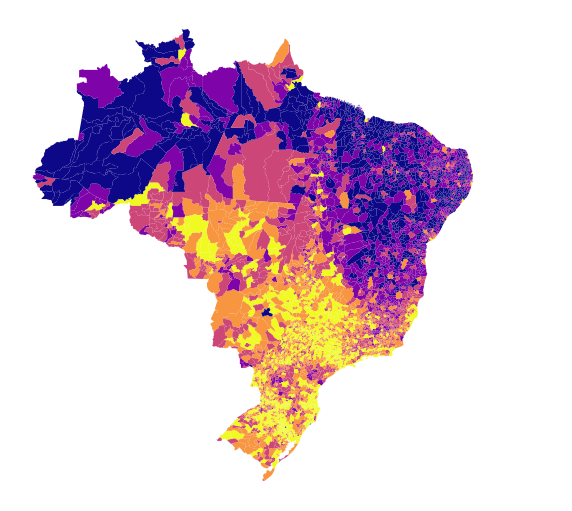
\includegraphics[width=0.30\textwidth]{img/br_3.png}}\hspace{0.2cm}
		\subfloat[Superfícies contínuas\label{fig:a}]{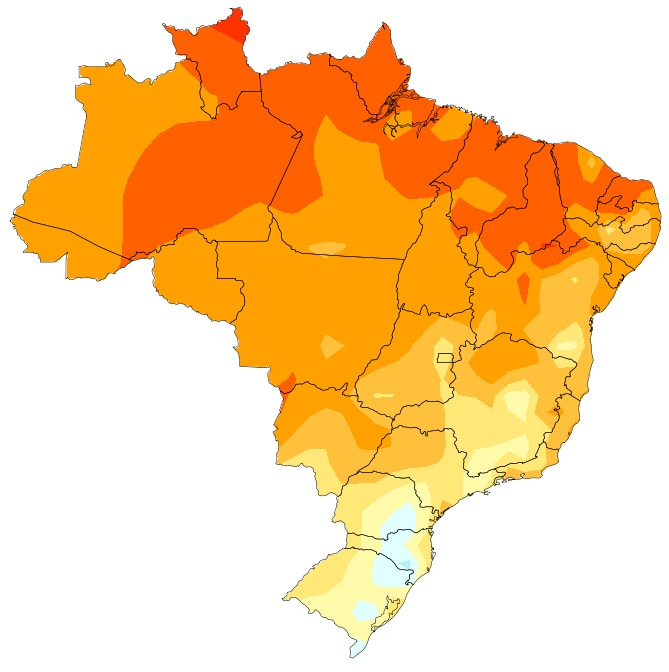
\includegraphics[width=0.25\textwidth]{img/br_geo.jpg}}\hspace{0.2cm}
		\subfloat[Eventos ou padrões pontuais\label{fig:c}]{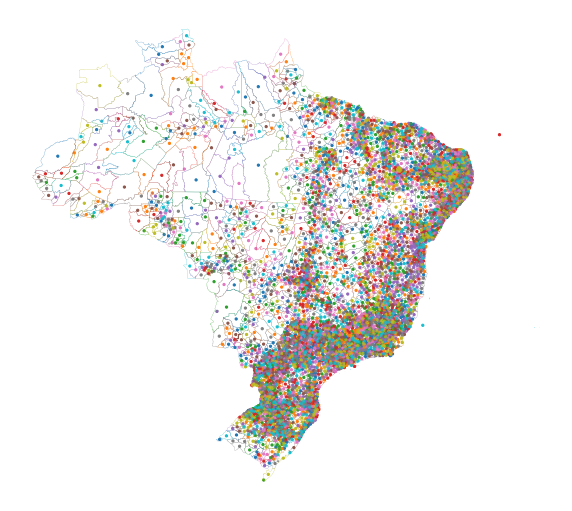
\includegraphics[width=0.30\textwidth]{img/inf_1.png}}
		\caption{Exemplos de dados espaciais}
		%\footnotesize{Fonte: (b) \url{revistapesquisa.fapesp.br}}
		\label{fig:2}
	\end{figure}
\end{frame}

\begin{frame}{Matriz de ponderação espacial}
	\begin{itemize}
	    \item É uma medida de proximidade entre as regiões.
	    \item Para um conjunto de $n$ áreas é definida como: 
	    \begin{align*}
        	\boldsymbol{W} =
	        \left[
	        \begin{array}{cccc}
		        w_{11} & w_{12} & \dots & w_{1n} \\
		        w_{21} & w_{22} & \dots &w_{2n} \\
		        \vdots & \vdots & \ddots & \vdots \\
		        w_{n1} & w_{n2} & \dots & w_{nn}\\
	        \end{array}
	        \right],
        \end{align*}
        \noindent Cada elemento $w_{ij}$ representa uma medida de proximidade entre as áreas $i$ e $j$. 
        \[
            w_{ij} = 
            \begin{cases}
                \text{1,} & \quad\text{se $i$ e $j$ são contíguos} \\
                \text{0,} & \quad\text{se $i$ e $j$ não são contíguos.}\\
            \end{cases}
        \]
        \noindent Por convenção, $w_{ij}=0,\quad \forall i=j$
	\end{itemize}
\end{frame}

\begin{frame}{Operador de defasagem espacial}
    \begin{itemize}
        \item \textbf{Defasagem}
    \end{itemize}
    $$y_{ij} \rightarrow y_{i-1,j},\text{ } y_{i,j-1},\text{ } y_{i+1,j},\dots$$  
    \begin{block}{}
        $$ \boldsymbol{W} \times y = Wy $$    
    \end{block}
    \noindent em que $\boldsymbol{W}$ é a matriz de pesos espaciais, $y$ é o vetor da variável e $Wy$ é a defasagem espacial da variável
    \begin{itemize}
        \item $Wy$ é a média do valor da variável nas regiões vizinhas se a matriz de pesos for normalizada nas linhas.
    \end{itemize}
\end{frame}

\begin{frame}{Autocorrelação espacial global}
	\begin{itemize}
		\item Um índice de autocorrelação espacial mede a associação espacial nos dados considerando o \textbf{local} e o \textbf{valor} da variável em estudo.
		\item Hipótese: Aleatoriedade na distribuição espacial da variável. 
	\end{itemize}
	
	\begin{figure}
		\centering
		\small
		\subfloat[Positiva\label{fig:a}]{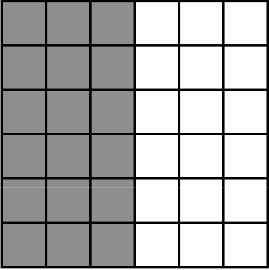
\includegraphics[width=0.15\textwidth]{img/autocor_pos.png}}\hspace{0.2cm}
		\subfloat[Nula\label{fig:b}]{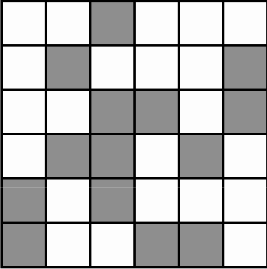
\includegraphics[width=0.15\textwidth]{img/autocor_null.png}}\hspace{0.2cm}
		\subfloat[Negativa\label{fig:c}]{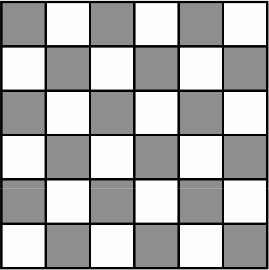
\includegraphics[width=0.15\textwidth]{img/autocor_neg.png}}
		\caption{Padrões de autocorrelação espacial}
		\small \textsuperscript {Fonte: Radil (2011)}
		\label{fig:1}
	\end{figure}
	\begin{itemize}
		\item É necessário usar uma estatística de teste para a aleatoriedade da distribuição espacial global da variável.
	\end{itemize}
\end{frame}

\begin{frame}{\textit{I} de Moran}
	O \textit{I} de Moran mede a relação do desvio padronizado de uma variável $z$ numa área $i$ com o desvio padronizado das 	áreas vizinhas $j$ para a mesma variável $z$ (ALMEIDA, 2012).
	
	\begin{block}{}
		\small
		\begin{align}
		\label{IMoran}
		I = \dfrac{n}{S_0} \dfrac{\displaystyle\sum_{i} \sum_{j} w_{ij} z_i z_j}{\displaystyle\sum_{i=1}^{n} z_i^2}.
		\end{align}
		\noindent \small em que $z_i = (x_i - \bar{x})$, $w_{ij}$ é uma medida de contiguidade entre $i$ e $j$,  $n$ é o número de regiões e $S_0$ é a soma dos pesos espaciais ($w_{ij}$)
	\end{block}	
\end{frame}

\begin{frame}{\textit{I} de Moran} %% Colocar mapa das apolices cotratadas
		\begin{figure}
			\centering
			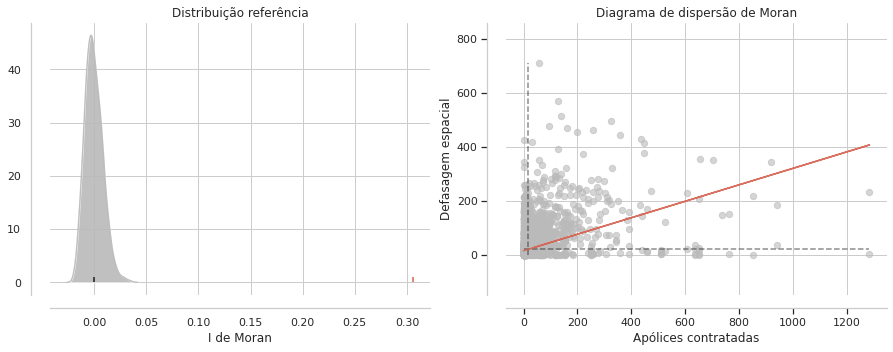
\includegraphics[width=0.8\textwidth]{img/i_de_moran.png}
			\caption{\textit{I} de Moran para Apólices contratadas}
		\end{figure}
\end{frame}

\begin{frame}{Autocorrelação espacial local}
	\begin{itemize}
		\item Estatísticas globais fornecem padrões de associação espacial em todo o conjunto de dados
		\item Medidas de autocorrelação local buscam identificar padrões no interior de uma região de estudo  
		\item Podem informar a existência de um \textit{cluster} de valores autocorrelacionados em nível local
		\item Podem informar sobre existência de \textit{outliers} locais
		\item Para Anselin (1995), um indicador local de associação espacial (\textit{LISA}) deve satisfazer a dois critérios:
		\vspace{0.25cm}
		\begin{enumerate}
			\item Deve indicar clusters espaciais estatisticamente significativos;
			\item A soma dos indicadores locais deve ser levar ao indicador global.
		\end{enumerate}
	\end{itemize}
\end{frame}

\begin{frame}{\textit{I} de Moran local}
	Um indicador local de associação espacial do tipo \textit{LISA} é o \textit{I} de Moran local que é expresso por: 
	\begin{block}{}
		\small
		\vspace{0.25cm}
		\begin{align*}
		I_i = z_i \sum_{j}^{} w_{ij} z_j,
		\end{align*}
		\noindent \small em que $z_i$ e $z_j$ são os valores da variável padronizada nas regiões $i$ e $j$, $w_{ij}$ é uma matriz de pesos espaciais.
	\end{block}	
\end{frame}

\begin{frame}{\textit{I} de Moran local}
	\begin{figure}
		\centering
		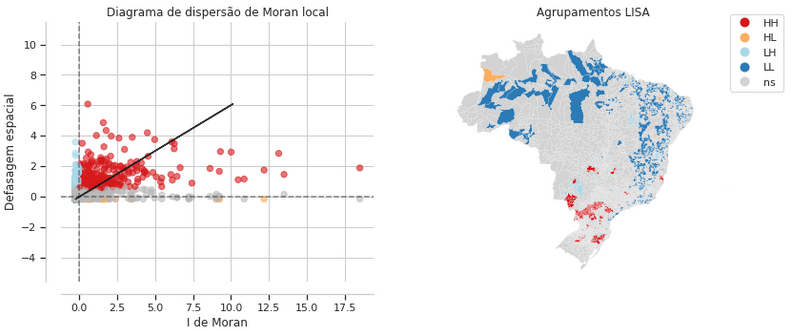
\includegraphics[width=0.8\textwidth]{img/lisa.png}
		\caption{$I$ de Moran local para Apólices contratadas}
		\label{fig:1}
	\end{figure}
\end{frame}

\begin{frame}{Modelando a dependência espacial}
    \begin{itemize}
        \item \textbf{Modelo Clássico de Regressão Linear}
        \vspace{0.5cm}
        \begin{block}{}
            $$y = X\beta + \varepsilon \quad \varepsilon\sim N(0,\sigma^2 \textbf{I})$$
        \end{block}
        \begin{itemize}
            \item \textbf{Processo a-espacial:}
        \end{itemize}
    \end{itemize}
    \begin{figure}
		\centering
		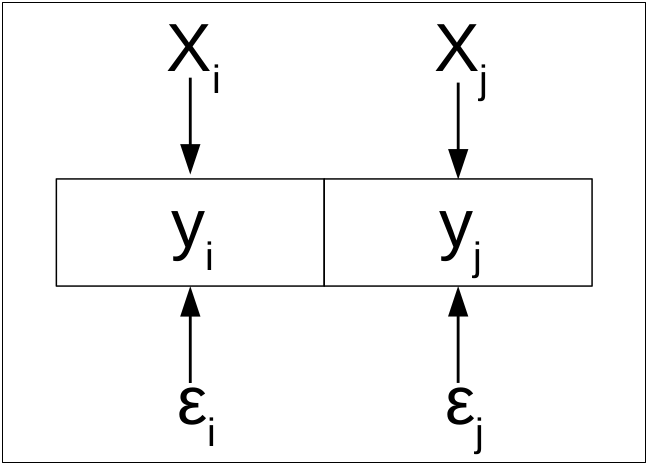
\includegraphics[width=0.25\textwidth]{img/reg_mcrl.png}
	\end{figure}
\end{frame}

\begin{frame}{Modelando a dependência espacial}
    \begin{itemize}
        \item \textbf{Modelo de defasagem espacial (\textit{SAR -- Spatial Auto Regressive})}
        \vspace{0.5cm}
        \begin{block}{}
            $$y = \rho Wy + \varepsilon \quad \text{ ou }\quad  y_i = \rho \sum_{j=1}^{n} w_{ij} y_j +  \varepsilon_i $$
        \end{block}
        \noindent em que $Wy$ é um vetor de defasagens espaciais (variável endógena)  e $\rho$ é o coeficiente auto-regressivo espacial. 
        \begin{itemize}
            \item \textbf{Processo espacial:}
        \end{itemize}
    \end{itemize}
    \begin{figure}
		\centering
		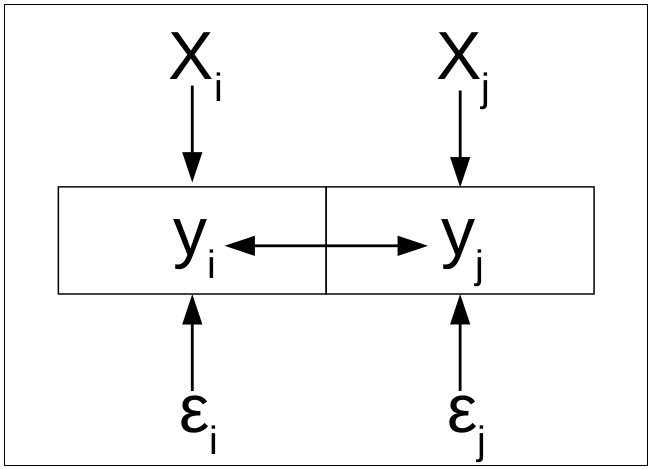
\includegraphics[width=0.25\textwidth]{img/reg_sar.png}
	\end{figure}
\end{frame}

\begin{frame}{Modelando a dependência espacial}
    \begin{itemize}
        \item \textbf{Modelo de defasagem espacial (\textit{SAR -- Spatial Auto Regressive})}
        
        \vspace{0.5cm}
        Incluindo variáveis exógenas (SAR misto)
        \vspace{0.2cm}
        \begin{block}{}
            $$y = \rho Wy + X\beta + \varepsilon  \quad \text{ ou }\quad  y_i = \rho \sum_{j=1}^{n} w_{ij} y_j + \sum_{j=1}^{p} x_{ij}\beta_j + \varepsilon_i$$
        \end{block}
        \noindent $X$ é a matriz de variáveis explicativas exógenas
    \end{itemize}
\end{frame}

\begin{frame}{Modelando a dependência espacial}
    \begin{itemize}
        \item \textbf{Modelo de erro auto-regressivo espacial (\textit{SEM -- Spatial Error Model})}
        \vspace{0.5cm}
        \begin{block}{}
            $$y = X\beta+ \xi \quad \text{ ou }\quad  y_i = \sum_{j=1}^{p} x_{ij}\beta_j + \xi_i$$  
            
            $$\xi = \lambda W \xi + \varepsilon \quad \text{ ou }\quad  \xi_i = \lambda \sum_{j=1}^{n} w_{ij} u_j + \varepsilon$$
        \end{block}
        \noindent 
        \begin{itemize}
            \item \textbf{Processo espacial:}
        \end{itemize}
    \end{itemize}
    \begin{figure}
		\centering
		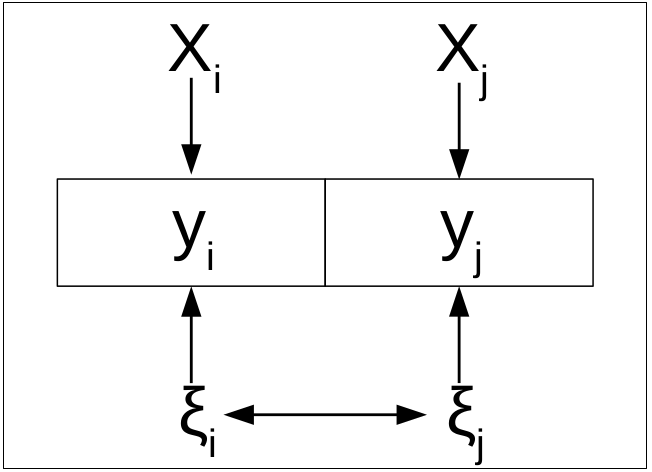
\includegraphics[width=0.25\textwidth]{img/reg_sem.png}
	\end{figure}
\end{frame}

\begin{frame}{Modelando a dependência espacial}
    \begin{itemize}
        \item \textbf{Modelo de defasagem espacial com erro autorregressivo espacial (\textit{SAC -- Spatial autoregressive combined})}
        
        \vspace{0.2cm}
        Há interação na variável de interesse $y$ e no erro $\xi$.
        %\vspace{0.5cm}
        \begin{block}{}
            $$y = \rho W_1y +  X\beta+ \xi \quad \text{ ou }\quad y_i = \rho \sum_{j=1}^{n} w_{1_{ij}} y_i + \sum_{j=1}^{p} x_{ij}\beta_j + \xi_i$$  
            
            $$\xi = \lambda W_2 \xi + \varepsilon \quad \text{ ou }\quad \xi_i = \lambda  \sum_{j=1}^{n} w_{2_{ij}} u_j + \varepsilon_1$$
        \end{block}
        \noindent $|\rho|<1$ e $|\lambda|<1$. 
    \end{itemize}
\end{frame}


\begin{frame}{Modelando a dependência espacial}
    \begin{itemize}
        \item \textbf{Modelo de defasagem espacial com erro autorregressivo espacial (\textit{SAC -- Spatial autoregressive combined})}
        \vspace{0.5cm}
        \begin{itemize}
            \item \textbf{Processo espacial:}
        \end{itemize}
    \end{itemize}
    \begin{figure}
		\centering
		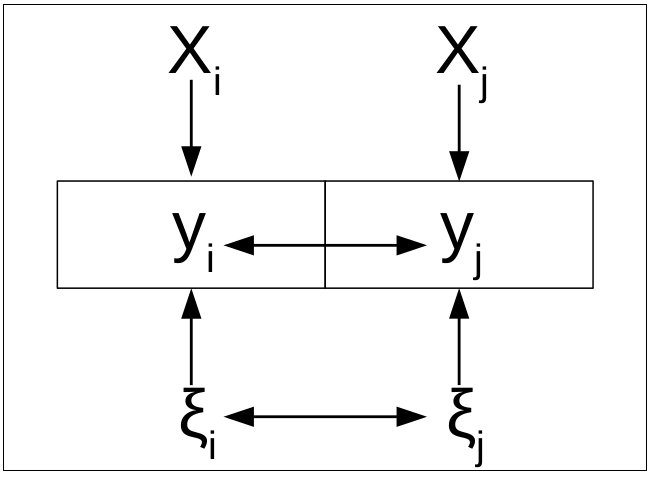
\includegraphics[width=0.25\textwidth]{img/reg_sac.png}
	\end{figure}
\end{frame}



\begin{frame}{Livros}
    \begin{figure}
		\centering
		\footnotesize
		\subfloat{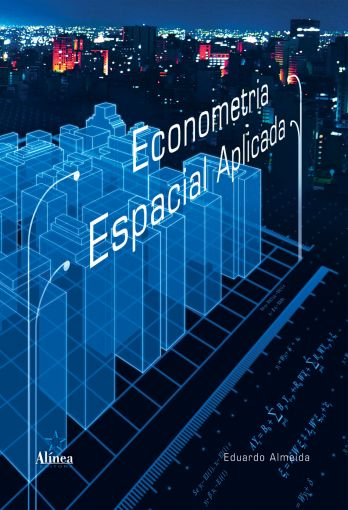
\includegraphics[height=5cm,keepaspectratio]{img/capa_almeida.jpg}}\hspace{0.3cm}
		\subfloat{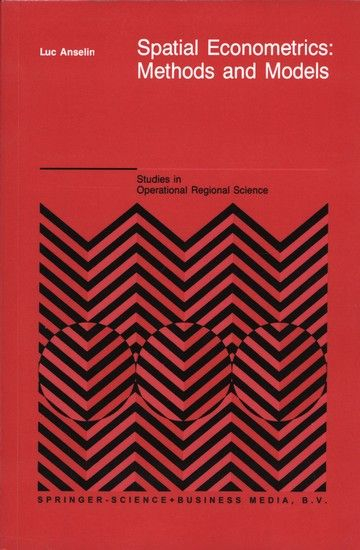
\includegraphics[height=5cm,keepaspectratio]{img/capa_anselin.jpg}}\hspace{0.3cm}
		\subfloat{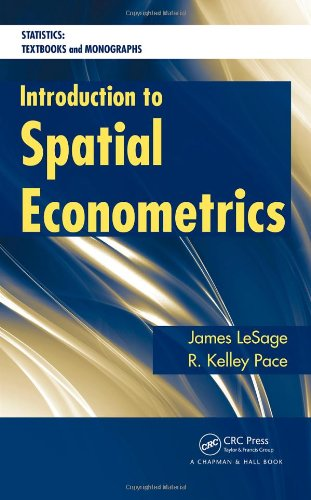
\includegraphics[height=5cm,keepaspectratio]{img/capa_lasage.jpg}}\hspace{0.3cm}
		\subfloat{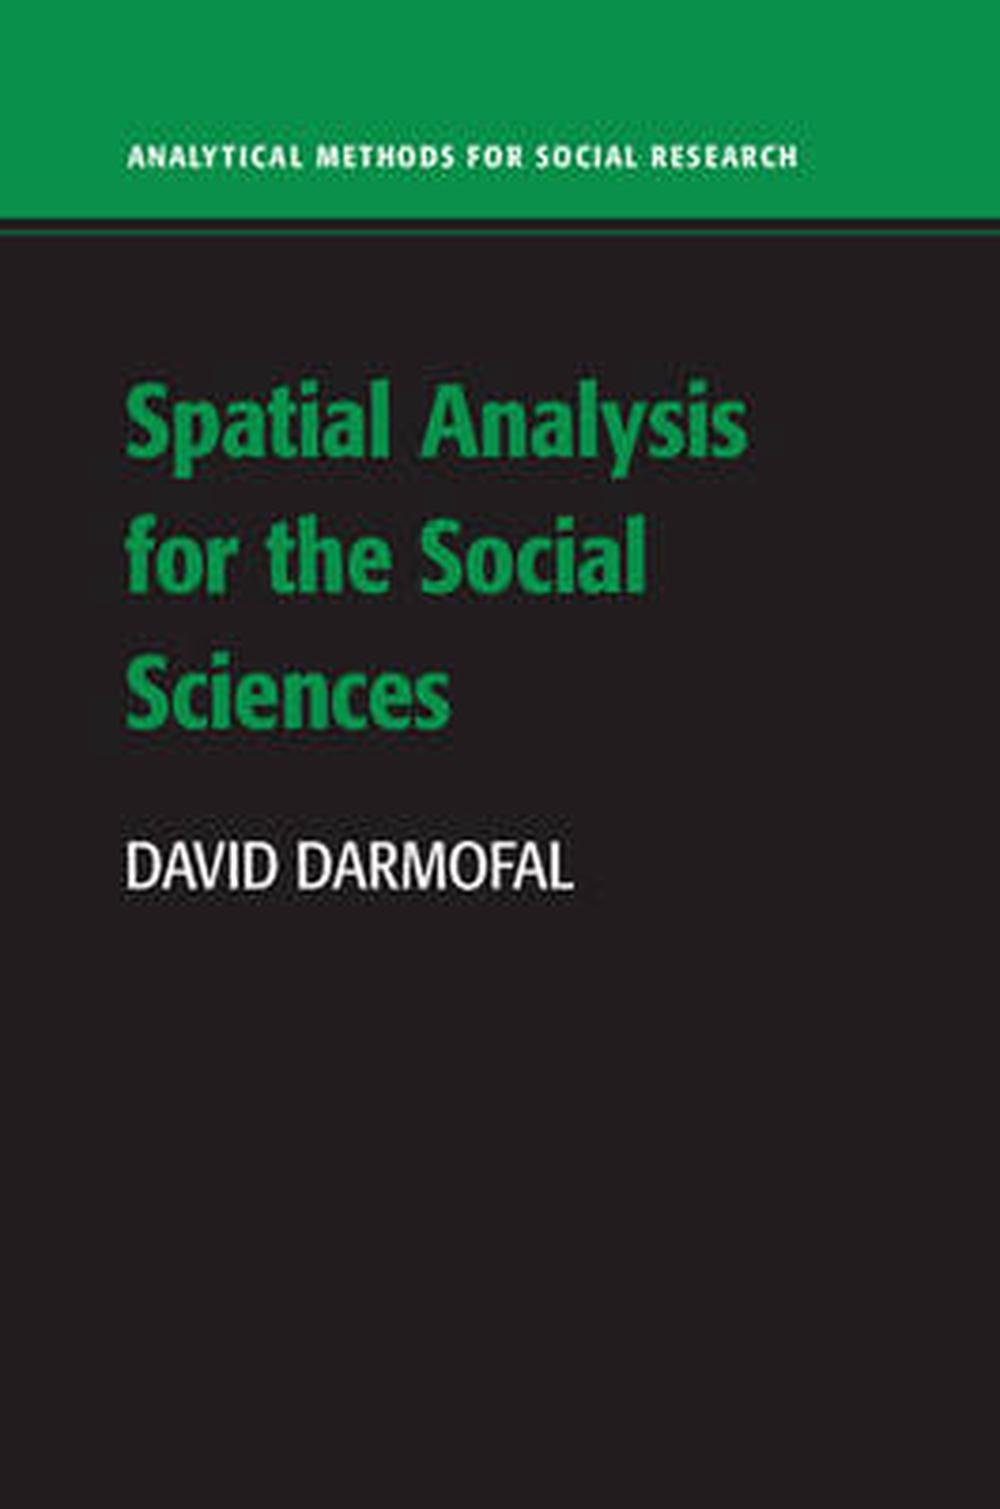
\includegraphics[height=5cm,keepaspectratio]{img/capa_darmofal.jpg}}\hspace{0.3cm}
	\end{figure}
\end{frame}


\begin{frame}{Links}
\begin{itemize}
    \item \url{https://darribas.org/gds_scipy16/}
    \item \url{https://spatial.uchicago.edu/}
    \item \url{https://www.youtube.com/user/GeoDaCenter}
    \item \url{https://geopandas.org/index.html}
    \item \url{https://geodacenter.github.io/index.html}
    \item \url{https://pysal.org/packages/}
    \item \url{https://www.liverpool.ac.uk/geographic-data-science/}
    \item \url{https://geographicdata.science/book/intro.html}
    \item \textbf{Repositório da apresentação no \textit{GitHub}:} \url{https://github.com/walefmachado/spreg_rural_insurance}
\end{itemize}
\end{frame}

\begin{frame}{Referências}
	\begin{flushleft}
			\footnotesize{

				{ALMEIDA, E. \textbf{Econometria Espacial Aplicada}. Campinas-SP: Alínea, 2012.}
				
				\vspace{0.25cm}
					
				{ANSELIN, L. Local indicatos of spatial association - LISA. \textbf{Geographical analysis}, v. 27, p. 93-115, 1995.}	

				\vspace{0.25cm}
				
				{JORDAHL, K. \textbf{GeoPandas}: Python tools for geographic data. 2014. Disponível em: \url{github.com/geopandas/geopandas}, Acesso em: 28 jul. 2020.}
				
				\vspace{0.25cm}
				
				{PYTHON. \textbf{The Python programming language}. Disponível em: \url{github.com/python/cpython}  Acesso em: 18 jul. 2017.}

				\vspace{0.25cm}

		    	{REY, S. J.; ANSELIN, L. PySAL: A Python library of spatial analytical methods.\textbf{ Review of Regional Studies}, v. 37, n. 1, p. 5–27, 2007.}
		    }
	\end{flushleft}
\end{frame}


\end{document}
